L'historien des sciences \som{pas seulement} peut se heurter à de nombreuses difficultés lors de son étude des diagrammes. La manière de les représenter diffère en fonction des conventions et des choix éditoriaux. Comparer les diagrammes à l'œil nu devient complexe même pour un spécialiste. \som{Attention à la formulation, ce n'est pas forcément vrai et la comparaison manuelle sera toujours plus précise que le travail automatique.}

\subsection{Les différentes conventions de représentation d'un diagramme}

Le travail de l'historien des sciences peut s'avérer compliqué lorsqu'un concept ou une démonstration est représentée de manière différente dans différents témoins. \som{Non} En effet, les conventions et les choix graphiques des diagrammes diffèrent en fonction de l'époque, de l'endroit et du sujet d'étude.

Michela Malpangotto étudie ce phénomène en s'appuyant sur l'exemple de l'œuvre de Théodose les \textit{Sphériques} écrite au Ier siècle avant notre ère. Il s'agit d'un texte fondamental dans l'étude de la géométrie sphérique qui est structuré en cinquante-neuf propositions et divisé en trois livres. Il fait partie de ce que l'on nomme la \og Petite astronomie \fg, un recueil d'ouvrages compilés par les Grecs afin de faciliter la compréhension de l'\textit{Almageste} de Ptolémée. Il a été étudié et transmis pendant près de dix siècles. La géométrie sphérique est définie de la manière suivante : \og La géométrie sphérique étudie la sphère comme un objet solide mais surtout comme contexte spatial des éléments qui interagissent sur elle dans un agencement tridimensionnel complexe. \fg Il est alors nécessaire de mettre au même niveau, le plan du diagramme et l'agencement spatial des objets autour de la sphère. Cette dernière est un objet solide mais elle est surtout un contexte spatial pour des arcs, des segments de droites et des cercles qui y sont déterminés par l'intersection de différents plans inclinés dans l'agencement spatial tridimensionnel. Cependant, le concept de sphère n'est pas représenté de la même manière chez tous les auteurs \footcite{malpangottoGraphicalChoicesGeometrical2010}. 

Dans la version grecque originale, illustré ici par le manuscrit \textit{Vat. Gr. 204}, les deux parties de l'œuvre sont séparées par le choix de l'iconographie des diagrammes. Dans la première partie, nous retrouvons des diagrammes dans lesquelles la sphère n'est pas représentée. Il y a seulement des cercles produits par l'intersection du plan incliné de différentes façons qui sont représentés de manière juxtaposée dans le plan du diagrammes. Les arcs ainsi que les segments linaires sont aplatis et les objets placés de l'autre côté de la sphère sont retournés dans le plan de la figure. La conséquence majeure de ce mode de représentation est la dépendance des diagrammes vis-à-vis du texte. Il est nécessaire de lire les explications pour comprendre le diagramme. Dans la seconde partie de l'œuvre, les diagrammes sont construits en utilisant la perspective. Nous pouvons donc observer les éléments géométriques interagir entre eux à l'intérieur de cette dernière \footcite{malpangottoGraphicalChoicesGeometrical2010}.  

En Italie, Platon de Tivoli a réalisé trois éditions de cette œuvre au XVIe siècle en s'appuyant sur une version arabo-latine médiévale. Il choisit de représenter les diagrammes de manière schématique et plane comme dans la première partie de la version grecque originale de l'œuvre. L'édition de Francesco Maurolico marque un tournant dans la transmission des \textit{Sphériques}. En effet, ce dernier fait le choix de travailler sur la surface de la sphère qui, mise en avant, devient le contexte réel dans lequel les éléments géométriques interagissent. Christophe Clavius, un mathématicien allemand adopte cette iconographie dans son édition de 1586 qui sert de base à la tradition moderne des \textit{Sphériques}\footcite{malpangottoGraphicalChoicesGeometrical2010}. 

\begin{figure}[H]
	\centering
	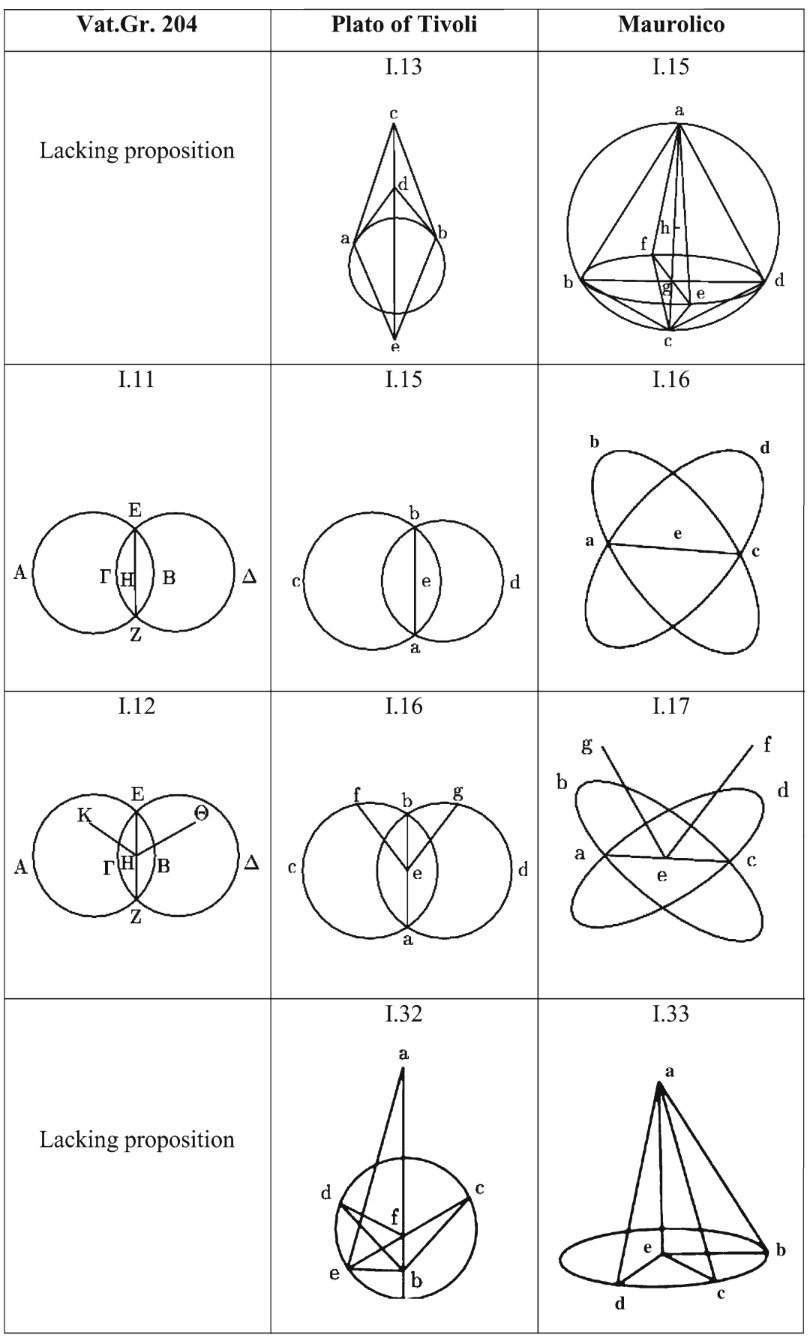
\includegraphics[width=0.6\linewidth]{images/conventions_diagrammes.png}
	\caption{Différentes conventions de représentation de diagrammes évoquées par Michela Malpangotto\footcite{malpangottoGraphicalChoicesGeometrical2010}}
	\label{fig:conventions}
\end{figure}


L'étude de Michela Malpangotto nous montre l'existence de nombreuses conventions graphiques de diagrammes pouvant être très différentes en fonction des éditeurs et des époques. Lorsque nous tentons de retracer la diffusion d'une œuvre à partir de ces diagrammes, il est important de prendre en compte ce paramètre. Néanmoins, ces différentes manières de représenter les diagrammes sont aussi en elles-mêmes les témoins de l'évolution d'un concept et donc par extension des connaissances scientifiques. \\

La question de la représentation des diagrammes est aussi une problématique que nous retrouvons dans les éditions plus contemporaines. 

\som{Mais du coup, les travaux cités comme exemple ont bel et bien été faits manuellement, sans que cela ne présente de difficulté particulière pour les chercheurs. Je pense que cette partie tombe à côté de la véritable problématique du projet, càd qu'il existe à travers les traditions un très grand nombre de manuscrits, qu'il est impossible sur le temps d'une vie de tous comparer précisément. De même, la question de la langue est importante, puisque c'est ça qui pose problème aux chercheurs qui sont rarement spécialistes de toutes les langues à la fois, et n'ont dans ce cas pas les outils pour faire des comparaisons à travers les traditions. Cela n'a rien à voir avec les conventions de représentation des diagrammes en elles-mêmes, d'autant qu'un outil numérique ne peut pas non plus faire cette comparaison automatiquement. On questionne donc la pertinence de l'argumentaire pour répondre à la problématique.}

\subsection{La modification des diagrammes dans les éditions modernes des sources scientifiques}

Les modifications que s'autorisent à faire les historiens et éditeurs contemporains peuvent rendre la comparaison avec les sources anciennes compliquée. Dans l'article déjà cité précédemment, Ken Saito étudie les éditions modernes des diagrammes astronomiques des \textit{Elements} d'Euclide. Il expose la problématique suivante : les diagrammes que nous voyons dans les éditions imprimées à partir du XIXe siècle sont très différents de ceux présents dans les manuscrits médiévaux. Pourtant les témoins datant du Moyen Age sont les meilleures versions, voire les seuls exemplaires d'œuvres antiques mathématiques en absence de manuscrit datant de cette époque. La version qui sert de base à beaucoup d'éditions contemporaines est celle de Heiberg datant de 1883-1888. Cependant, ce dernier s'est contenté de recopier les diagrammes de Ferdinand August simplifiés dans un but pédagogique dans son édition datant des années 1820 \footcite{saitoTraditionsDiagramTradition2012}. Se pose alors la question des conventions d'édition. Deux points de vue s'opposent. Nous avons d'abord celui de la maison d'édition \textit{Les Belles Lettres} décrit dans leur \textit{Règles et recommandations pour les éditions critiques} qui explique qu'il est nécessaire de reproduire les diagrammes aussi précisément que possible sans essayer de les corriger ou de les modifier. Michael Hunter, lui, défend plutôt l'idée selon laquelle il est acceptable que les diagrammes soient redessinés pour que l'intention originelle de l'auteur soit transmise au lecteur\footcite{jardineCriticalEditingEarlyModern2010}.\\

Ces différentes manières de représenter un même diagramme peuvent poser problème aux chercheurs lorsque ces derniers cherchent à établir des liens entre les différents témoins d'une même œuvre ou tradition. Même pour un spécialiste qui connaît parfaitement les différentes conventions, identifier et comparer chaque diagramme dans plusieurs témoins peut s'avérer être très chronophage.

\som{Pourquoi on voudrait comparer sources anciennes et contemporaines ? Ce n'est le sujet d'aucun projet de recherche cités dans le mémoire, et encore une fois, un chercheur qui le souhaite peut tout à fait faire cette comparaison. Ça n'a rien à voir avec les modifications que font les éditeurs et les historiens. Ce que AIKON/EIDA questionne, c'est l'absence de normes d'édition et de vocabulaire standardisé pour l'édition des diagrammes.}